\chapter{Kapitel 2: Klassen}
\section{Elfen}
\textit{Hochnäsig aber freundlich.}

\subsection*{Namen}
Wenn ein Elf erwachsen wird sucht er sich einen neuen Namen aus. Davor wird er nach dem Kindernamen gerufen.\\
\textbf{Kindernamen:}\\
Ara, Bryn, Del, Eryn, Faen, Innil, Lael, Mella, Naill, Naeris, Phann, Rael, Rinn, Sai, Syllin, Thia, Vall\\
\textbf{Männliche Erwachsenennamen:}\\
Adran, Aelar, Armil, Arannis, Aust, Beiro, Berrian, Carric, Enialis, Erdan, Erevan, Calinndan, Hadarai, Heian, Himo, Immeral, Ivellios, Laucian, Mindartis, Paelias, Peren, Quariom, Riardon, Rolen, Soveliss, Thamior, Tharivol, Theren, Varis\\
\textbf{Weibliche Erwachsenennamen:}\\
Adrie, Althaea, Anastrianna, Andrastem Antinua, Bethrynna, Birel, Caelynn, Drusilia, Enna, Felosial, Ielenia, Jelenneth, Keyleth, Leshanna, Lia, Meriele, Mialee, Naivara, Quelenna, Quillathe, Sariel, Shanairra, Shava, Silaqui, Theirastra, Thia, Vadannia, Valenthe, Xanaphia

\subsection*{Alter}
Körperliche Reife, wie bei Menschen, schließt Lebenserfahrung mit ins Erwachsenwerden ein. Erwachsenenalter: 100 Jahre. Kann bis zu 750 Jahre alt werden.

\subsection*{Gesinnung}
Eine sanftere Ausprägung des Chaos. Schätzen und verteidigen Freiheit aller. rücksichtslos und heimtückisch

\subsection*{Größe}
Etwas kleiner als Menschen, weit unter 150cm und knapp über 180cm

\subsection*{Gewicht}
100-145 Pfund

\subsection*{Attributserhöhung}
$Geschicklichkeitswert + 2$

\subsection*{Bewegungsrate}
9 Meter / 30 Fuß / 3 Felder

\subsection*{Fähigkeiten}
\begin{itemize}
	\item Dunkelsicht
	\item Geschärfte Sinne
	\item Feenblut
	\item Trance
\end{itemize}

\subsection*{Sprachen}
\begin{itemize}
	\item Gemeinsprache, Elfisch
	\subitem lesen, schreiben, sprechen
\end{itemize}

\subsection*{Unterarten}
Zu Informationen und Werten zu den Unterarten siehe PH.
\begin{itemize}
	\item Hochelfen
	\item Waldelfen
	\item Dunkelelfen
\end{itemize}

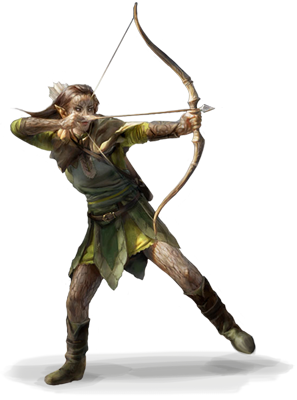
\includegraphics[width=\textwidth / 3]{img/elf} %70% der Textbreite

% ####################################################
%
% ####################################################

\newpage
\section{Halblinge}

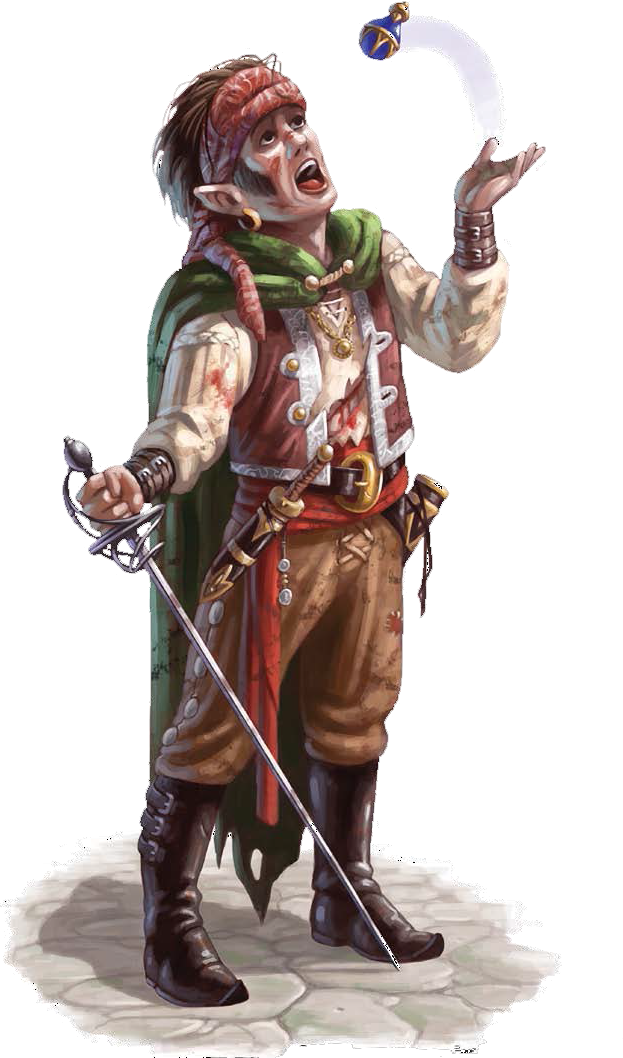
\includegraphics[width=\textwidth / 3]{img/halbling}

\textit{Umgänglich und positiv.}

\subsection*{Namen}
Jeder Halbling besitzt einen Vornamen, Familiennamen und möglicherweise einen Spitznamen. Bei Familiennamen handelt es sich oft um Spitznamen die so treffend waren, dass sie über Generationen hinweg weiter gegeben wurden\\
\textbf{Männliche Vornamen:}\\
Alton, Ander, Cade, Coorin, Eldon, Errich, Finan, Garret, Lindal, Lyle, Merric, Milo, Osborn, Perrin, Reed, Roscoe, Wellby\\
\textbf{Weibliche Vornamen:}\\
Andry, Bree, Callie, Cora, Euphemia, Jillian, Kithri, Lavinia, Merla, Nedda, Paela, Portia, Seraphina, Sheana, Trym, Vani, Verna\\
\textbf{Familiennamen:}\\
Buschsammler, Dickdorn, Fallkraut, Grünflasche, Goldbarren, Hochhügel, Hügelspitz, Strammgurt, Teeblatt, Unterast

\subsection*{Alter}
Ist mit 20 Jahre erwachsen. lebt ca. 150 Jahre.

\subsection*{Gesinnung}
Rechtschaffen gut. Mitfühlend, warmherzig und freundlich. Tollerieren keine Form der Unterdrückung.

\subsection*{Größe}
~ 90cm groß

\subsection*{Gewicht}
40 Pfund

\subsection*{Attributserhöhung}
$Geschicklichkeitswert + 2$

\subsection*{Bewegungsrate}
7,5 Meter / 22,5 Fuß / 2 Felder

\subsection*{Fähigkeiten}
\begin{itemize}
	\item Halblingsglück
	\item Tapferkeit
	\item Halblingsgewandheit
\end{itemize}

\subsection*{Sprachen}
\begin{itemize}
	\item Halblingisch, Gemeinsprache
	\subitem lesen, schreiben, sprechen
\end{itemize}

\subsection*{Unterarten}
Zu Informationen und Werten zu den Unterarten siehe PH.
\begin{itemize}
	\item Leichtfüße
	\item Stämmige
\end{itemize}

% ####################################################
%
% ####################################################

\newpage
\section{Menschen}

\textit{Jedermanns zweitbester Freund.}

\subsection*{Namen}
Keine spezifischen Namen. Für Inspiration können Namen aus den 9 Ethischen Gruppen verwendet werden. \textit{siehe Seite 28 im PH.}

\subsection*{Alter}
Ist mit 20 Jahre erwachsen. lebt wenigger als ein Jahrhundert.

\subsection*{Gesinnung}
Keine bestimmte Gesinnung.

\subsection*{Größe}
Kaum 150cm bis 180cm

\subsection*{Gewicht}
Schwankt stark

\subsection*{Attributserhöhung}
$Jeder Attributswert + 1$

\subsection*{Bewegungsrate}
9 Meter / 30 Fuß / 3 Felder

\subsection*{Fähigkeiten}
/

\subsection*{Sprachen}
\begin{itemize}
	\item Gemeinsprache, andere Sprache
	\subitem lesen, schreiben, sprechen
	\item Lernen häufig die Sprache mit denen sie am meisten zu tun haben.
	\item wollen belesen wirken und streuen Fremdworte in ihre Sprache.
\end{itemize}

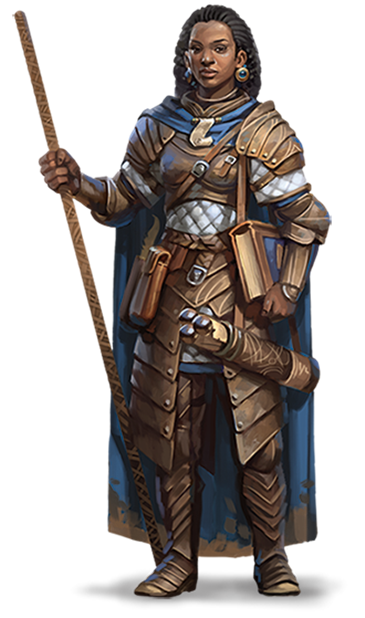
\includegraphics[width=\textwidth / 3]{img/human}


% ####################################################
%
% ####################################################

\newpage
\section{Zwerge}

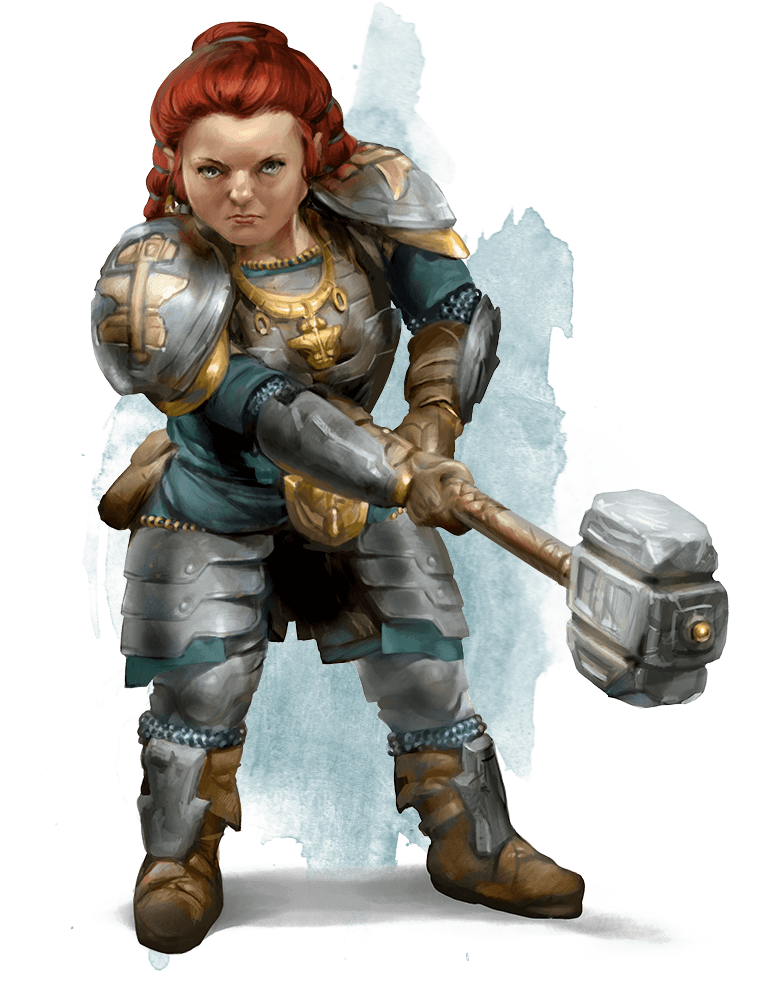
\includegraphics[width=\textwidth / 3]{img/zwerg}

\textit{Baut erst langsam Vertrauen auf und ist nachtragend wegen gutem Gedächtnis}

\subsection*{Namen}
Jeder Zwerg bekommt den Namen von dem Klanältesten verliehen. Bringt er Schande über diesen Namen wird es ihm per Gesetz verboten einen anderen Namen als diesen zu tragen.\\
\textbf{Männliche Vornamen:}\\
ADrik, Allberich, Baeren, Barendd, Bottor, Bruenor, Dain, Darrak, Delg, Eberk, Einkil, Fargrim, Flint, Gardain, Harbek, Kildrak, Morgran, Orsik, Oskar, Rangrim, Rurik, Taklinn, Thoradin, Thorin, Tordek, Traubon, Travok, Ulfgar, Veit, Vondal
\\
\textbf{Weibliche Vornamen:}\\
Amber, Artin, Audhild, Bardryn, Dagnal, Diesa, Eldeth, Falkrunn, Finellen, Gunndola, Gurdis, Helja, Hlin, Kathra, Kristryd, Ilde, Liftrasa, Mardred, Riswynn, Sannl, Torbera, Torgga, Vistra\\
\textbf{Klannamen:}\\
Balderk, Heldenhammer, Starkamboss, Dankil, Feuerschmiede, Frostbart, Gorunn, Holderheck, Eisenfaust, Loderr, Lutgehr, Rumnaheim, Strakeln, Torunn, Ungart

\subsection*{Alter}
Altern so schnell wie Menschen. Werden mit 50 noch als Jung angesehen. Werden ca. 350 Jahre alt.

\subsection*{Gesinnung}
Glauben an eine Durchstrukturierte Gesellschaft, also rechtschaffend. Glauben dass jeder es verdient hat an einer gerechten Ordnung teilzu haben.
\subsection*{Größe}
120cm-150cm

\subsection*{Gewicht}
150 Pfund

\subsection*{Attributserhöhung}
$Konstitutionswert + 2$

\subsection*{Bewegungsrate}
7,5 Meter / 22,5 Fuß / 2 Felder

Wird nicht durch das Tragen von schwerer Rüstung reduziert.

\subsection*{Fähigkeiten}
\begin{itemize}
	\item Dunkelsicht
	\item Zwergische Unverwüstbarkeit
	\item Zwergisches Kampftraining
	\item Handwerkliches Geschick
	\item Steingespür
\end{itemize}

\subsection*{Sprachen}
\begin{itemize}
	\item Zwergisch, Gemeinsprache
	\subitem lesen, schreiben, sprechen
\end{itemize}

\subsection*{Unterarten}
Zu Informationen und Werten zu den Unterarten siehe PH.
\begin{itemize}
	\item Gebirgszwerg
	\item Hügelzwerg
\end{itemize}

% ####################################################
%
% ####################################################

\newpage
\section{Drachenblütige}

\subsection*{Namen}
\subsection*{Alter}
\subsection*{Gesinnung}
\subsection*{Größe}
\subsection*{Gewicht}
\subsection*{Attributserhöhung}
\subsection*{Bewegungsrate}
\subsection*{Fähigkeiten}
\subsection*{Sprachen}
\subsection*{Unterarten}

% ####################################################
%
% ####################################################

\newpage
\section{Gnome}

\subsection*{Namen}
\subsection*{Alter}
\subsection*{Gesinnung}
\subsection*{Größe}
\subsection*{Gewicht}
\subsection*{Attributserhöhung}
\subsection*{Bewegungsrate}
\subsection*{Fähigkeiten}
\subsection*{Sprachen}
\subsection*{Unterarten}


% ####################################################
%
% ####################################################

\newpage
\section{Halbelfen}

\subsection*{Namen}
\subsection*{Alter}
\subsection*{Gesinnung}
\subsection*{Größe}
\subsection*{Gewicht}
\subsection*{Attributserhöhung}
\subsection*{Bewegungsrate}
\subsection*{Fähigkeiten}
\subsection*{Sprachen}
\subsection*{Unterarten}


% ####################################################
%
% ####################################################

\newpage
\section{Halborks}

\subsection*{Namen}
\subsection*{Alter}
\subsection*{Gesinnung}
\subsection*{Größe}
\subsection*{Gewicht}
\subsection*{Attributserhöhung}
\subsection*{Bewegungsrate}
\subsection*{Fähigkeiten}
\subsection*{Sprachen}
\subsection*{Unterarten}

% ####################################################
%
% ####################################################

\newpage
\section{Tiefling}

\subsection*{Namen}
\subsection*{Alter}
\subsection*{Gesinnung}
\subsection*{Größe}
\subsection*{Gewicht}
\subsection*{Attributserhöhung}
\subsection*{Bewegungsrate}
\subsection*{Fähigkeiten}
\subsection*{Sprachen}
\subsection*{Unterarten}
